\documentclass[12pt]{article}
\usepackage[final]{graphicx}
\usepackage[utf8]{inputenc}

% Set margins
\usepackage[a4paper, left=1in,right=1in,top=1in,bottom=1in]{geometry}

% Add bibliography
\usepackage[backend=bibtex8,autocite=superscript,style=numeric,citestyle=numeric]{biblatex}
\addbibresource{final.bib}
\renewbibmacro{in:}{}

% Make hyperlinks prettier
\usepackage[colorlinks,urlcolor=blue]{hyperref}
\urlstyle{same}

% Header settings  
\usepackage{fancyhdr}
\pagestyle{fancy}
\fancyhf{}
\rhead{Paul Ruess}
% \chead{Paul Ruess}
\lhead{Real-time Flood Prediction: Improvements on Rating Curve Relationships}
\rfoot{Page \thepage}

% Enable floating and wrapped figures
\usepackage{wrapfig}
\usepackage{floatrow}

% Decrease spacing between list items
\usepackage{enumerate}
\usepackage{enumitem}
\setlist[description]{itemsep=0mm}

% Force table caption to top
\usepackage{floatrow}
\floatsetup[table]{capposition=top}

% Bold math symbols
\usepackage{amsmath}
\usepackage{bm}

% Subfigures
% used for rating curve figure
\usepackage{subcaption}

% Tweak abstract
\renewenvironment{abstract}
 {\small
  \begin{center}
  \bfseries \abstractname\vspace{-.5em}\vspace{0pt}
  \end{center}
  \list{}{%
    \setlength{\leftmargin}{0mm}% <---------- change margins
    \setlength{\rightmargin}{\leftmargin}%
  }%
  \item\relax}
 {\endlist}

% Minimize white space
\usepackage[compact]{titlesec}

% Change section titles
\usepackage{titlesec}
\titleformat*{\section}{\bfseries\large}
\titleformat*{\subsection}{\bfseries\normalsize}

% Keywords command
\providecommand{\keywords}[1]{\textbf{\textit{Keywords---}} #1}

% Make my name bold in references
\newcommand{\makeauthorbold}[1]{%
\DeclareNameFormat{author}{%
  \ifnumequal{\value{listcount}}{1}
    {\ifnumequal{\value{liststop}}{1}
      {\expandafter\ifstrequal{##1}{#1}{\textbf{##1\addcomma\addspace ##4\addcomma\isdot}}{##1\addcomma\addspace ##4\addcomma\isdot}}
      {\expandafter\ifstrequal{##1}{#1}{\textbf{##1\addcomma\addspace ##4}}{##1\addcomma\addspace ##4}}}
    {\ifnumless{\value{listcount}}{\value{liststop}}
      {\expandafter\ifstrequal{##1}{#1}{\textbf{\addcomma\addspace ##1\addcomma\addspace ##4}}{\addcomma\addspace ##1\addcomma\addspace ##4}}
      {\expandafter\ifstrequal{##1}{#1}{\textbf{\addcomma\addspace ##1\addcomma\addspace ##4\addcomma\isdot}}{\addcomma\addspace ##1\addcomma\addspace ##4\addcomma\isdot}}%
    }%
}%
}
\makeauthorbold{Ruess}

% Title
\title{\vspace*{-0.0in}{\bfseries\large A Comparison of Rating Curve Generation Methodologies}\vspace{-11pt}}
\author{{\textit{\normalsize Paul Ruess}}}
\date{\vspace{-30pt}}

\begin{document}
% \section*{\centerline{Research Proposal}}
\maketitle

\begin{abstract} % Get them interested! 
Flooding is the most impactful natural disaster worldwide: ``since 1995, floods have accounted for 47\% of all weatherrelated disasters, affecting 2.3 billion people''.\cite{disaster2015} In response to this need, ongoing research applying the Height Above Nearest Drainage (HAND) methodology to flood mapping is underway, yet this approach cannot realistically be implemented until accurate stage-discharge relationship exist for all stream reaches.\cite{nfiehand} This research will investigate potential trends in rating curve formulation in an attempt to improve national-scale rating curve generalizations for the $\sim$2.7 million stream reaches in the Continental United States (CONUS). This will ultimately enable the use of the National Water Model (NWM) to inform flood extent predictions that can be communicated to citizens and first responders, potentially saving lives.

\end{abstract}

\keywords{Flood Prediction, Rating Curve, Stage Height} % Trim this to one line
% \vspace{-11pt}

\section*{Introduction} % Introduce the topic you are interested in.
% National Water Model, HAND methodology, Manning's equation, 
As described by the Office of Water Prediction (OWP), the newly released NWM is ``a hydrologic model that simulates observed and forecast streamflow for the CONUS'', increasing the number of stream forecasting points from $\sim$3,600 to $\sim$2.7 million \cite{nwmsummary}.\autocite{nwmsummary} This enormous increase in coverage has tremendous implications for enabling real-time flood forecasting, yet further research is needed to accurately convert from streamflows to flood depths and from flood depths to flood extents. In order to generate truly informative flood predictions, this research will focus on the first of these two tasks: improving streamflow-to-flood-depth conversions through a statistical comparison of various rating curves. 

\section*{Research Questions} % One or several research questions you want to address as part of your project. 

% \begin{figure}[h!]
%   \centering
%   \includegraphics[keepaspectratio, width=.8\textwidth]{rc__comid_5781369_from_0_to_100.png}
%   \caption{Rating Curves for COMID 5781369}\label{fig:rc_all_5781369}
% \end{figure}

\begin{wrapfigure}{R!}{0.4\textwidth}
  \centering
  \vspace{-22pt}
  \includegraphics[keepaspectratio, width=1\textwidth]{rc__comid_5781369_from_0_to_100.png}
  \caption{Rating Curves for COMID 5781369} \label{fig:rc_all_5781369}
\end{wrapfigure}

The primary objective of this paper is to assess differences between three different rating curves: a HAND rating curve, a United States Geological Survey (USGS) rating curve, and a so-called "Resistance Function" rating curve derived from various HEC-RAS (Hydrologic Engineering Center's River Analysis System) rating curves (see Figure \ref{fig:rc_all_5781369} for details). This assessment will ideally inform improvements to HAND-generated rating curves for all $\sim$2.7 million stream reaches in the nation. 

\section*{Hypotheses} % Formulate a research hypothesis for each of the research questions to be tested as part of your analysis. 

The expectation is that a statistically-significant rating curve can be determined from an aggregate of the available data, improving stream-reach flood extent mapping. It is further expected that USGS rating curves will be consistent with HEC-RAS rating curves derived from nearby cross-sections. 

\section*{Data}

Before exploring the available, an introduction to the rating curve methodologies here used is necessary. A rating curve describes the relationship between volumetric discharge (ie. streamflow) and river stage (ie. height of a river measured above the lowest point in the cross-section) for a stream reach. Various methodologies exist for mathematically creating rating curves. In this paper, the rating curve methodology based on Manning's equation will be used to statistically generalize a best-fit rating curve for each of the $\sim$2.7 million stream reaches in the CONUS. Manning's equation has been used in this paper in order to maintain consistency with the methods used to generate HAND rating curves. Manning's equation is described as follows: 

\begin{equation}
Q = \frac{k}{n}A_wH_R^\frac{2}{3}S_0^\frac{1}{2}
\end{equation}
where: 
\begin{description}
  \item[\bm{$Q$}] is the discharge [L\textsuperscript{3}/T];
  \item[\bm{$A_w$}] is the cross-sectional wetted area [L\textsuperscript{2}];
  \item[\bm{$H_R$}] is the hydraulic radius [L];
  \item[\bm{$S_0$}] is the channel bed slope at constant water depth [L/L];
  \item[\bm{$n$}] is the so-called Manning's roughness coefficient [T/L\textsuperscript{1/3}]. 
  \item[\bm{$k$}] is a conversion factor, 1.0 for SI units and 1.49 for English units.
\end{description}

Using Manning's equation, a rating curve can only be created if the discharge and height (included in the area term) are related, requiring $A_w$, $H_R$, $S_0$, and $n$ to be known. According to the OWP, ``all [NWM] configurations provide streamflow for 2.7 million river reaches and other hydrologic information on 1km and 250m grids'' \cite{nwmsummary}. As such, once a rating curve is known for each stream reach, discharges provided by the NWM can be used to programatically predict flood extents for the entire nation. This is the true objective of, and justification for, this particular research. 

$S_0$ can be retrieved from the NHDPlusV2 dataset \cite{nhdplusv2}, while the HAND methodology (currently in development by Xing Zheng) can  be used to determine $A_w$ and $H_R$ at each depth interval (ie. every 1 foot). Given these hydraulic properties, the only remaining variable required is manning's roughness coefficient, $n$. Manning's roughness can either be retrieved from existing data sources (such as USGS field measurements or HEC-RAS models), or --- as in the case of the HAND rating curves --- can be reasonably approximated as 0.05 (see Table \ref{table:roughness}). Finally, Manning's equation can be used to compute discharge for all depth intervals, enabling the generation of rating curves. 

\begin{table}[H]
\centering
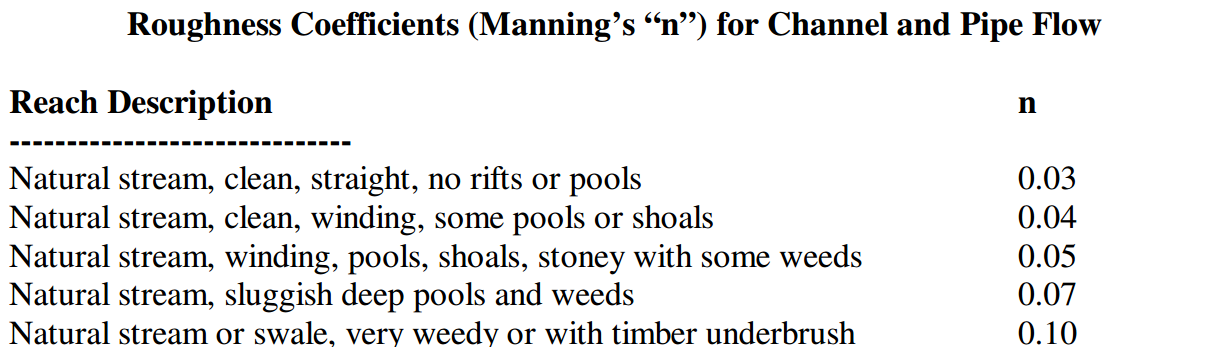
\includegraphics[keepaspectratio, width=1\textwidth]{n_vals.png}
\caption{Commonly accepted Manning's $n$ values \cite{roughnesstable}}\label{table:roughness}
\end{table}

For this project, HAND rating curve parameters were programatically retrieved from a NetCDF file containing all HAND data for Onion Creek (provided by Xing Zheng, the creator of the national HAND raster). HAND rating curves were also provided as a benchmark for assessing potential improvements; these are the rating curves using a Manning's roughness of 0.05. 

Regarding the other two datasets, USGS rating curves have been retrieved from the USGS Water Watch Customized Rating Curve Builder \cite{usgswaterwatch}, and HEC-RAS cross-sections along with their associated Manning's roughness values ($n$) have been retrieved for the Onion Creek watershed from Xing Zheng's masters thesis. Collectively, these two datasets, alongside the HAND rating curves, are sufficient data to meaningfully compare rating curve construction methodologies to assess which approaches could best be generalized at a national scale \cite{xingms}. 

A more detailed description of these three methodologies will now be explained... 

\subsection*{HAND Rating Curves}

The HAND methodology determines a height value for each 10m x 10m raster grid-cell based on that cell's nearest stream reach, determined by following the path of steepest descent using a 10m x 10m Digital Elevation Model (DEM). As a result, the HAND raster represents the stage height requirement for each grid-cell to become inundated. For example, a HAND value of 20 ft means that the grid-cell in question is 20 ft above it's nearest stream reach, meaning that once the stream reaches a stage height of 20 ft, that particular grid-cell will become inundated. 

The HAND methodology is intended primarily for flood inundation mapping (ie. given a stage-height, a flood extent map can be produced by showing which grid-cells are inundated); however, by using an assumed maximum depth, the HAND method can also be used to approximate $A_w$ and $H_R$ for each depth interval. This process, and the process for collecting the additional remaining parameters, is as follows (see Figure \ref{fig:nfiehand} for details): 

% \begin{description}
%   \item[\bm{$A_w$}] Calculated for each assumed stage height (ie. depth interval) and a channel width calculated as $(number~of~inundated~cells)*(cell~width)$.
%   \item[\bm{$H_R$}] Calculated by adding the channel top-width plus the channel side-length, where top-width is calculated using total flood surface-area divided by river length, and channel side-length is calculated using the triangular geometry of each depth interval. Channels are assumed to have a trapezoidal geometry. 
% \end{description}

As mentioned, the data needed to construct a HAND rating curve is the following: 

\begin{description}
  \item[\bm{$A_w$}] Calculated using stage height and channel width.
  \item[\bm{$H_R$}] Calculated using channel top-width and channel side-length, assuming a trapezoidal channel geometry. 
  \item[\bm{$S_0$}] Retrieved from the NHDPlusV2 dataset using stream reach COMIDs \cite{nhdplusv2}.
  \item[\bm{$n$}] Assumed as 0.05 for this study, based on commonly accepted values (see Table \ref{table:roughness}).
\end{description}

\begin{figure}[b]
  \centering
  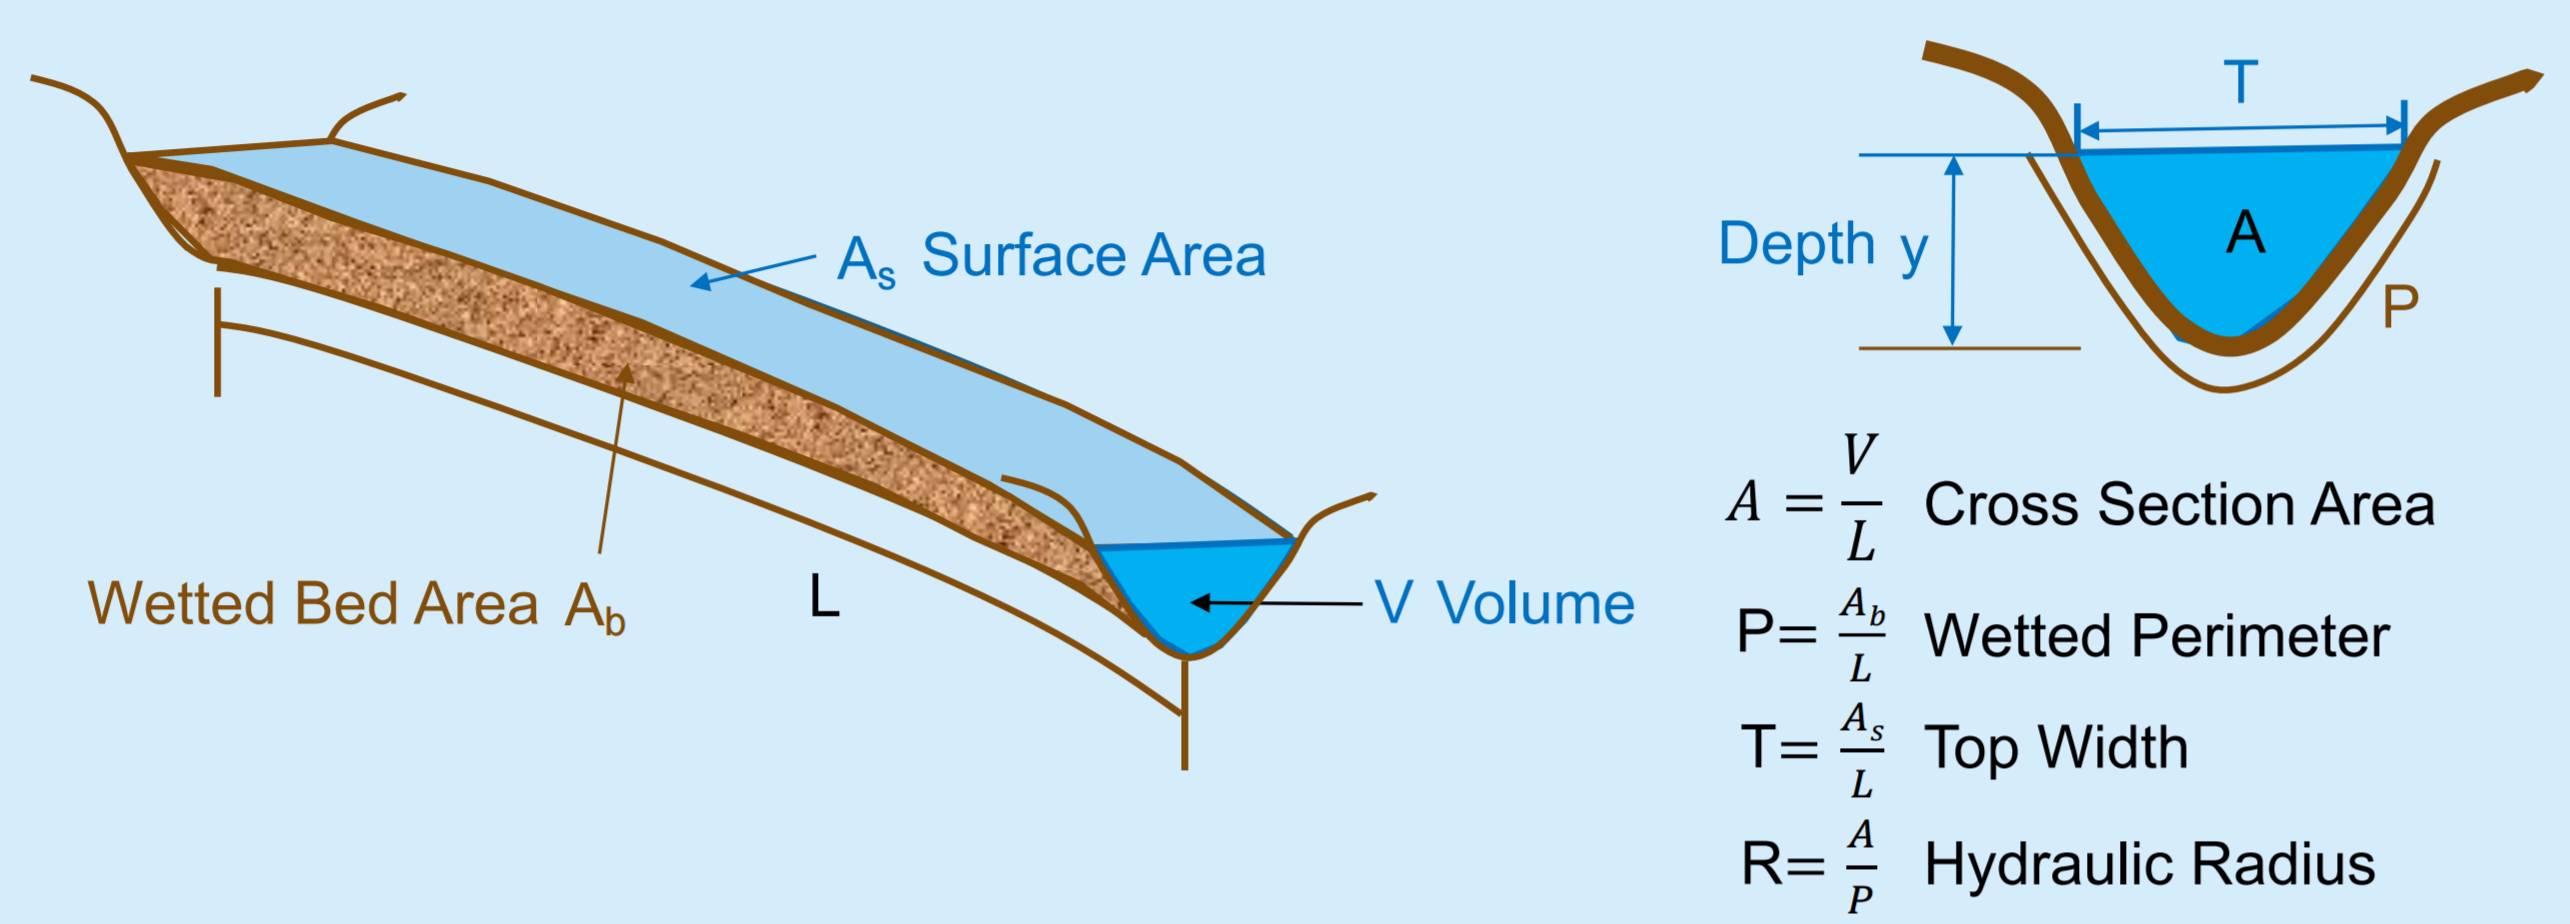
\includegraphics[keepaspectratio, width=.8\textwidth]{hydroparams.png}
  \caption{Hydraulic Parameter Relationships \cite{nfiehand}}\label{fig:nfiehand}
\end{figure}

As mentioned previously, HAND rating curve parameters and the rating curves themselves were read from a NetCDF file. Notably, the accuracy of these rating curves is questionable due to DEM imperfections: DEMs are generally constructed with the use of remote sensing technologies, which frequently fail to penetrate through water surfaces. This discrepancy introduces potentially faulty errors to the HAND-based rating curve creation previously described. Further complications arise due to the Manning's roughness assumption of 0.05 for all streams; clearly this ignores the physical characteristics of the stream, and therefore these streams are relatively meaningless overall. This research therefore intends to ultimately determine a potential correction for these HAND rating curves, seeing as this is the sole dataset --- of those used in this study --- covering all $\sim$2.7 million stream reaches in the CONUS. 

\subsection*{USGS Rating Curves}

Thankfully, the United States Geological Survey (USGS) has meticulously characterized rating curves for $\sim$6,600 stream reaches based on in-situ measurements of stage and discharge, alongside field approximations of Manning's roughness \cite{usgswaterwatch}. The level of detail of these rating curves is very high, and the USGS has been defining rating curves for many years, so these USGS rating curves are generally considered the industry standard. 

The biggest downside to the USGS rating curves is their relative scarcity. Clearly USGS rating curves can not be used for national-scale flood extent predictions as-is, though ideally there are ways to intelligently extrapolate these USGS rating curves to the remaining $\sim$2.7 million stream reaches. 

\subsection*{HEC-RAS Rating Curves}

HEC-RAS is a hydraulic modeling software developed by the United States Army Corps of Engineers, with many applications to flood modeling. In order to generate HEC-RAS rating curves, a HEC-RAS model containing hydraulic properties along each modeled reach must be created. Luckily, a HEC-RAS model of Austin is publicly available from the City of Austin, and Xing Zheng's Master's Thesis focused on "flooding" this model for five critical discharges: 10-year, 25-year, 50-year, 100-year, and 500-year flood events; these results were saved in two .csv files. Using this data, theoretical rating curves can be fitted for each HEC-RAS rating curve, describing the stage-discharge relationship at each cross-section along a stream reach. This analysis can then repeated for all reaches covered by the Austin HEC-RAS model, and this methodology could easily be re-applied for any existing HEC-RAS model with cross-sectional data. 

\section*{Study Area}

In order to analyze these rating curves at a reasonable scale, the Onion Creek watershed (just South-West of Austin) was selected as a study area (Figure \ref{fig:onioncreekwatershed}). Details in this watershed are included in the form of both 2- and 3-dimensional maps of three particular stream reaches with COMID values 5781369, 5781373, and 5781407. The importance of selecting these particular stream reaches depends primarily on the placement of the USGS gage: COMID 5781369 has a USGS gage near the beginning of the reach, COMID 5781373 has a USGS gage near the end of the reach, and COMID 5781407 has a USGS gage near the center of the reach; this aided in the assessment of the relationship between HEC-RAS rating curves as compared to the nearby USGS rating curves (based on cross-section location along the stream reach). It is also important to note that these reaches all have a fairly high cross-section density, enabling a more dense analysis (because there are more HEC-RAS rating curve data available). 

\begin{figure}[t]
  \centering
  \includegraphics[keepaspectratio, width=.8\textwidth]{studyarea.png}
  \caption{Study Area: Onion Creek Watershed}\label{fig:onioncreekwatershed}
\end{figure} 

\subsection*{Details: COMIDs 5781369, 5781373, and 5781407}

COMID 5781369 has a length of 15,521 ft, and the USGS gage is relatively close to the front of the stream reach (Figure \ref{fig:5781369_studyarea}). Furthermore, there is a fairly large variation in cross-sectional geometry (as can be seen from the 3D map). This variation is important for understanding scaling trends. COMID 5781373, however, has a length of 25,803 ft and with a USGS gage relatively close to the end of the stream reach (Figure \ref{fig:5781373_studyarea}). Finally, COMID 5781407 has a USGS gage right in the middle, and an even longer length of 32,175 ft. 

\begin{figure}[h!]
\makebox[\linewidth][c]{
\begin{subfigure}{0.75\textwidth}
  \centering
  \includegraphics[keepaspectratio, width=\textwidth]{5781369_2d.jpg}
  \caption{COMID 5781369 2-Dimensional Map}\label{fig:5781369_2d.jpg}
\end{subfigure}
% \hspace*{\fill}
\begin{subfigure}{0.25\textwidth}
  \centering
  \includegraphics[keepaspectratio, width=\textwidth]{5781369_3d.jpg}
  \caption{COMID 5781369 3-Dimensional Map}\label{fig:5781369_3d.jpg}
\end{subfigure}
% \hspace*{\fill}
}
\caption{COMID 5781369 Study Area} \label{fig:5781369_studyarea}
\end{figure}

\begin{figure}[h!]
\makebox[\linewidth][c]{
\begin{subfigure}{0.42\textwidth}
  \centering
  \includegraphics[keepaspectratio, width=\textwidth]{5781373_2d.jpg}
  \caption{COMID 5781373 2-Dimensional Map}\label{fig:5781373_2d.jpg}
\end{subfigure}
% \hspace*{\fill}
\begin{subfigure}{0.3\textwidth}
  \centering
  \includegraphics[keepaspectratio, width=\textwidth]{5781373_3d.jpg}
  \caption{COMID 5781373 3-Dimensional Map}\label{fig:5781373_3d.jpg}
\end{subfigure}
% \hspace*{\fill}
}
\caption{COMID 5781373 Study Area} \label{fig:5781373_studyarea}
\end{figure}

\begin{figure}[h!]
\makebox[\linewidth][c]{
\begin{subfigure}{0.65\textwidth}
  \centering
  \includegraphics[keepaspectratio, width=\textwidth]{5781407_2d.jpg}
  \caption{COMID 5781407 2-Dimensional Map}\label{fig:5781407_2d.jpg}
\end{subfigure}
% \hspace*{\fill}
\begin{subfigure}{0.3\textwidth}
  \centering
  \includegraphics[keepaspectratio, width=\textwidth]{5781407_3d.jpg}
  \caption{COMID 5781407 3-Dimensional Map}\label{fig:5781407_3d.jpg}
\end{subfigure}
% \hspace*{\fill}
}
\caption{COMID 5781407 Study Area} \label{fig:5781407_studyarea}
\end{figure}

\section*{Methods}

In order to reasonably compare these HEC-RAS rating curves to the HAND and USGS rating curves, a reach-averaged representation of all HEC-RAS rating curves must first be derived. This relationship was derived as a so-called "resistance function" by first computing the Manning's roughness for each discharge for every stage-height between 0 and 82 (this extent of stage heights was chosen for consistency with the HAND rating curve stage-height spread). Once all of these Manning's roughness values were computed, they could be averaged for each stage-height and a representative discharge for each stage-height could be determined, resulting in a "resistance function" rating curve for that particular reach as derived from the HEC-RAS cross-section rating curves. 

In an effort to better understand the spread of these discharges with respect to stage-height, multiple box-plots were plotted for every stage height for all of the reaches in the study area with HEC-RAS cross-section data. In the results section, three examples are shown displaying this spread of discharge values. 

Importantly, in order to retrieve data values from the HEC-RAS rating curves at various 1-ft stage-height intervals, these HEC-RAS rating curves had to be fitted. Rating curves often follow a power-law fit (as can be seen visually from the raw curve data, and as is generally accepted by the literature \cite{ahgdingman}), and thus this fitting was used for the purposes of this paper. A linear fit could feasibly have been used (with larger error), but this would have led to very iffy values beyond the final HEC-RAS data point (ie. the "500-year flood stage"). 

A power-law relationship is defined by the following equation: 

\begin{equation}
y = Ax^B
\end{equation}
where A and B are constants describing the function in question. 

In order to fit a (linear) regression, the HEC-RAS rating curves were all programatically transformed to a natural log - natural log relationship. Following this transformation, a linear fitting of the data was possible, and this fit enabled a computation of the slope (B) and the intercept (logA) of each line. With a bit more manipulation, each HEC-RAS line was successfully fitted with a Power-Law line, enabling queries on the HEC-RAS dataset at all stage-heights. 

\section*{Results}

\subsection*{Box Plot}

Box plots were created for all COMIDs in the Onion Creek watershed which contained HEC-RAS cross-sections. Boxplots for three of the COMIDs --- 5781369, 5781373, and 5781407 --- are shown below to visually display the spread of the data. 

\begin{figure}[h!]
\makebox[\linewidth][c]{
\begin{subfigure}{0.33\textwidth}
  \centering
  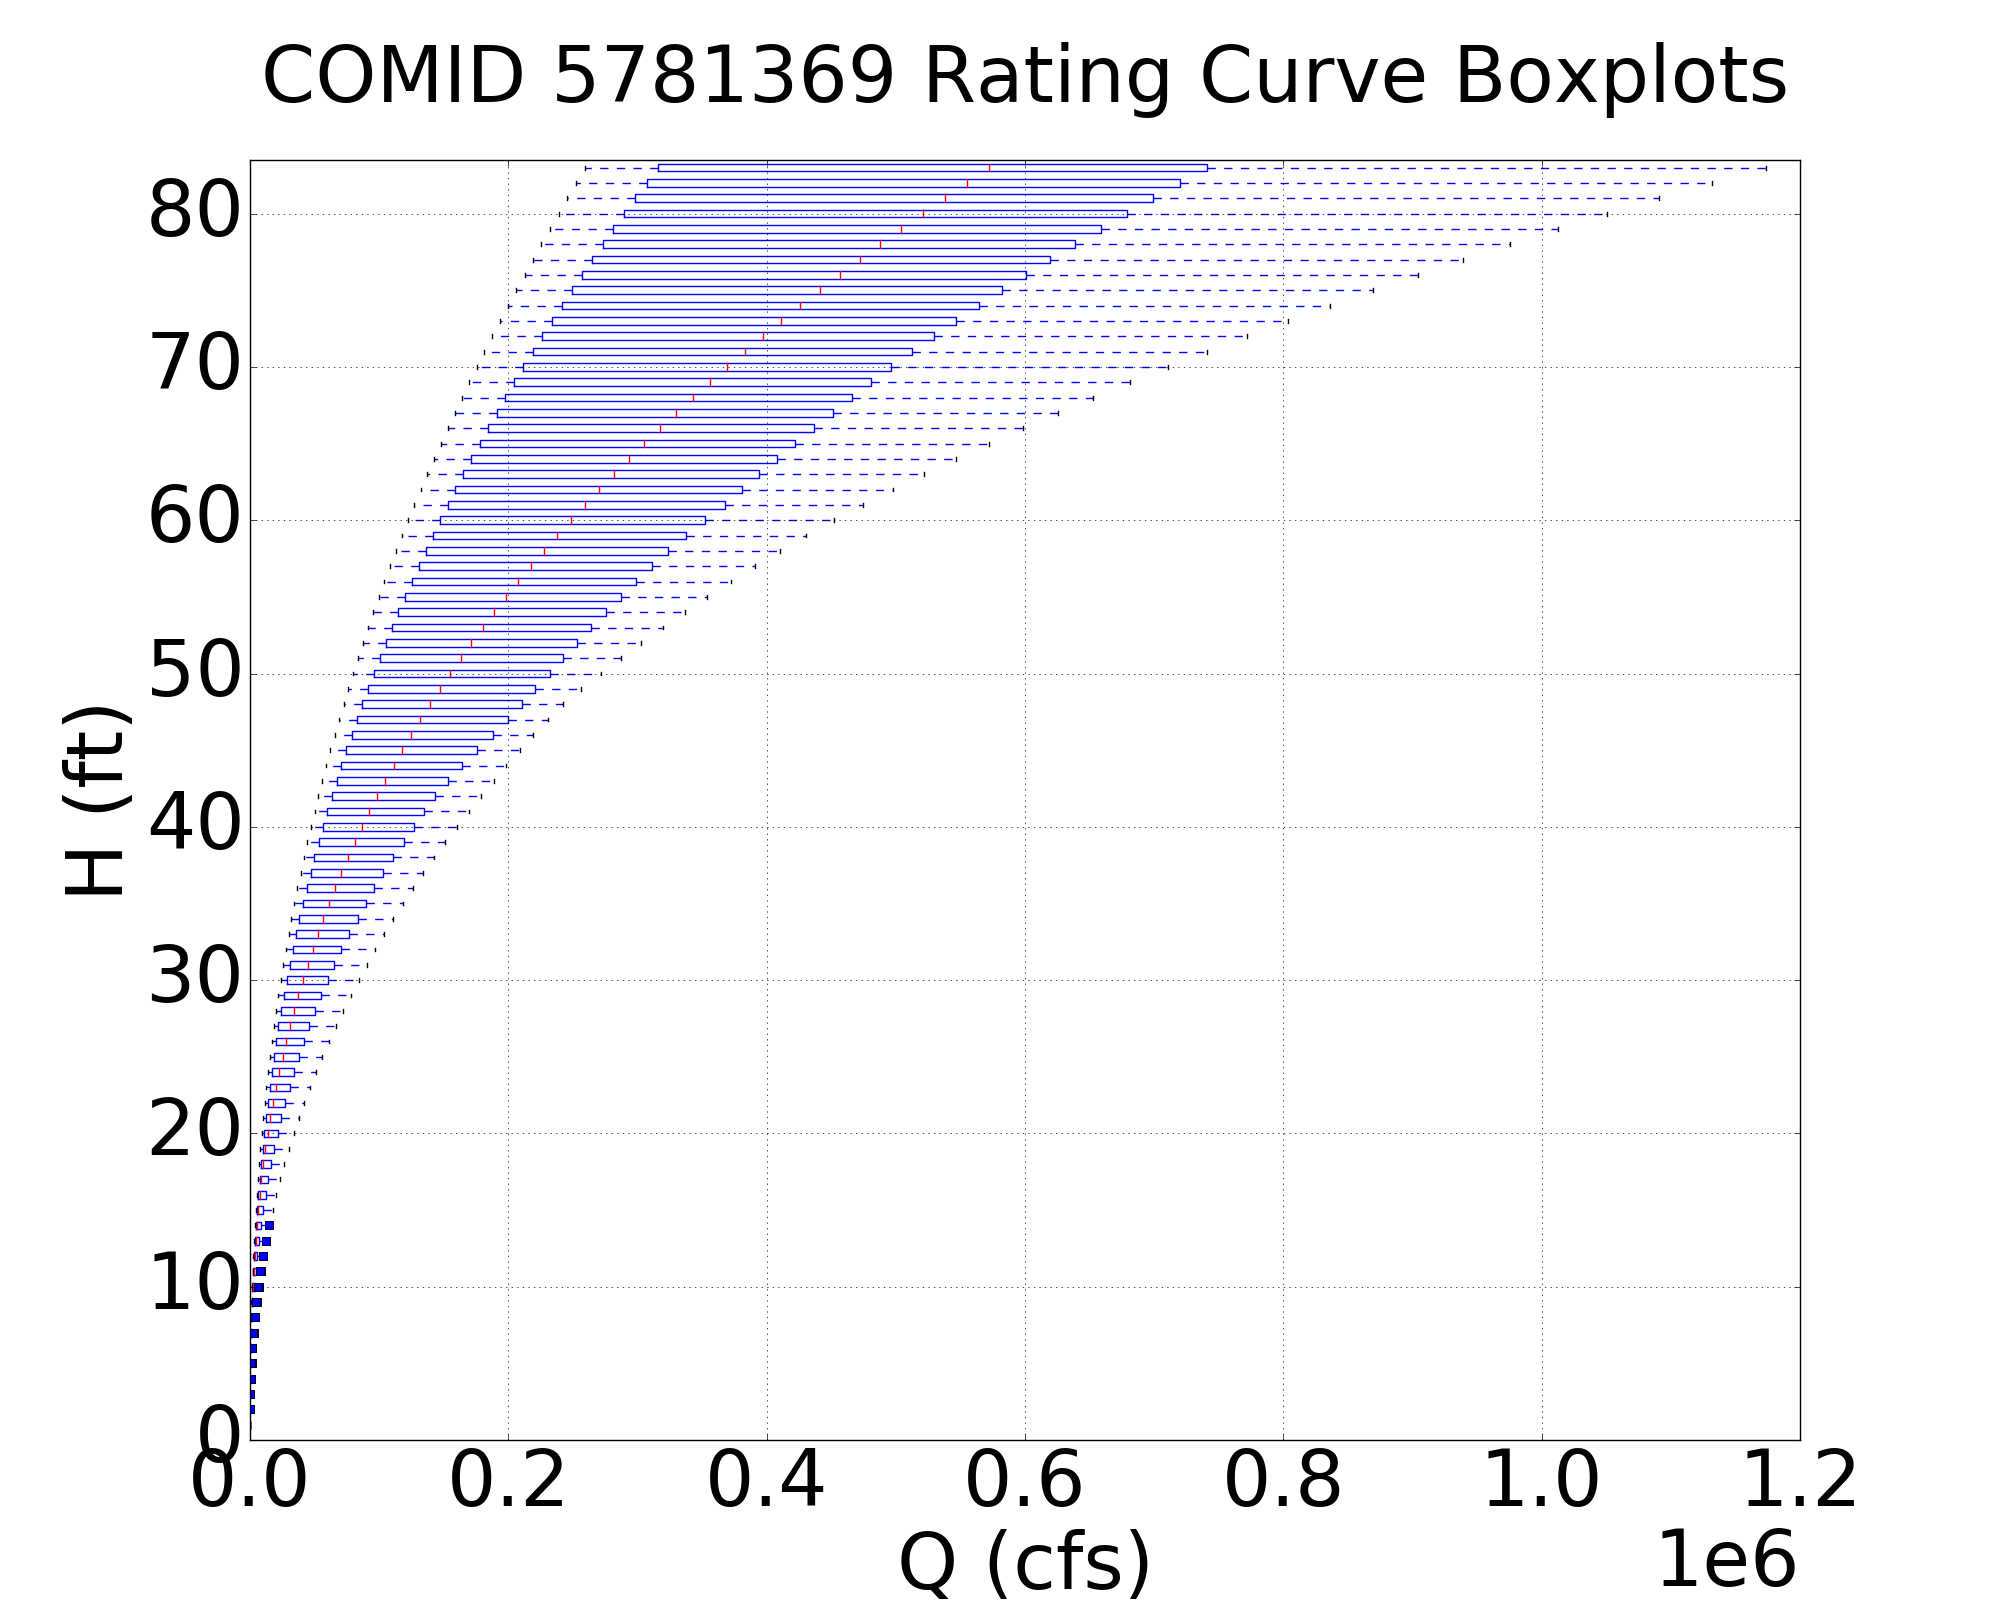
\includegraphics[keepaspectratio, width=\textwidth]{multi_boxplot_5781369.png}
  \caption{COMID 5781369 Boxplots}\label{fig:5781369_box}
\end{subfigure}
% \hspace*{\fill}
\begin{subfigure}{0.33\textwidth}
  \centering
  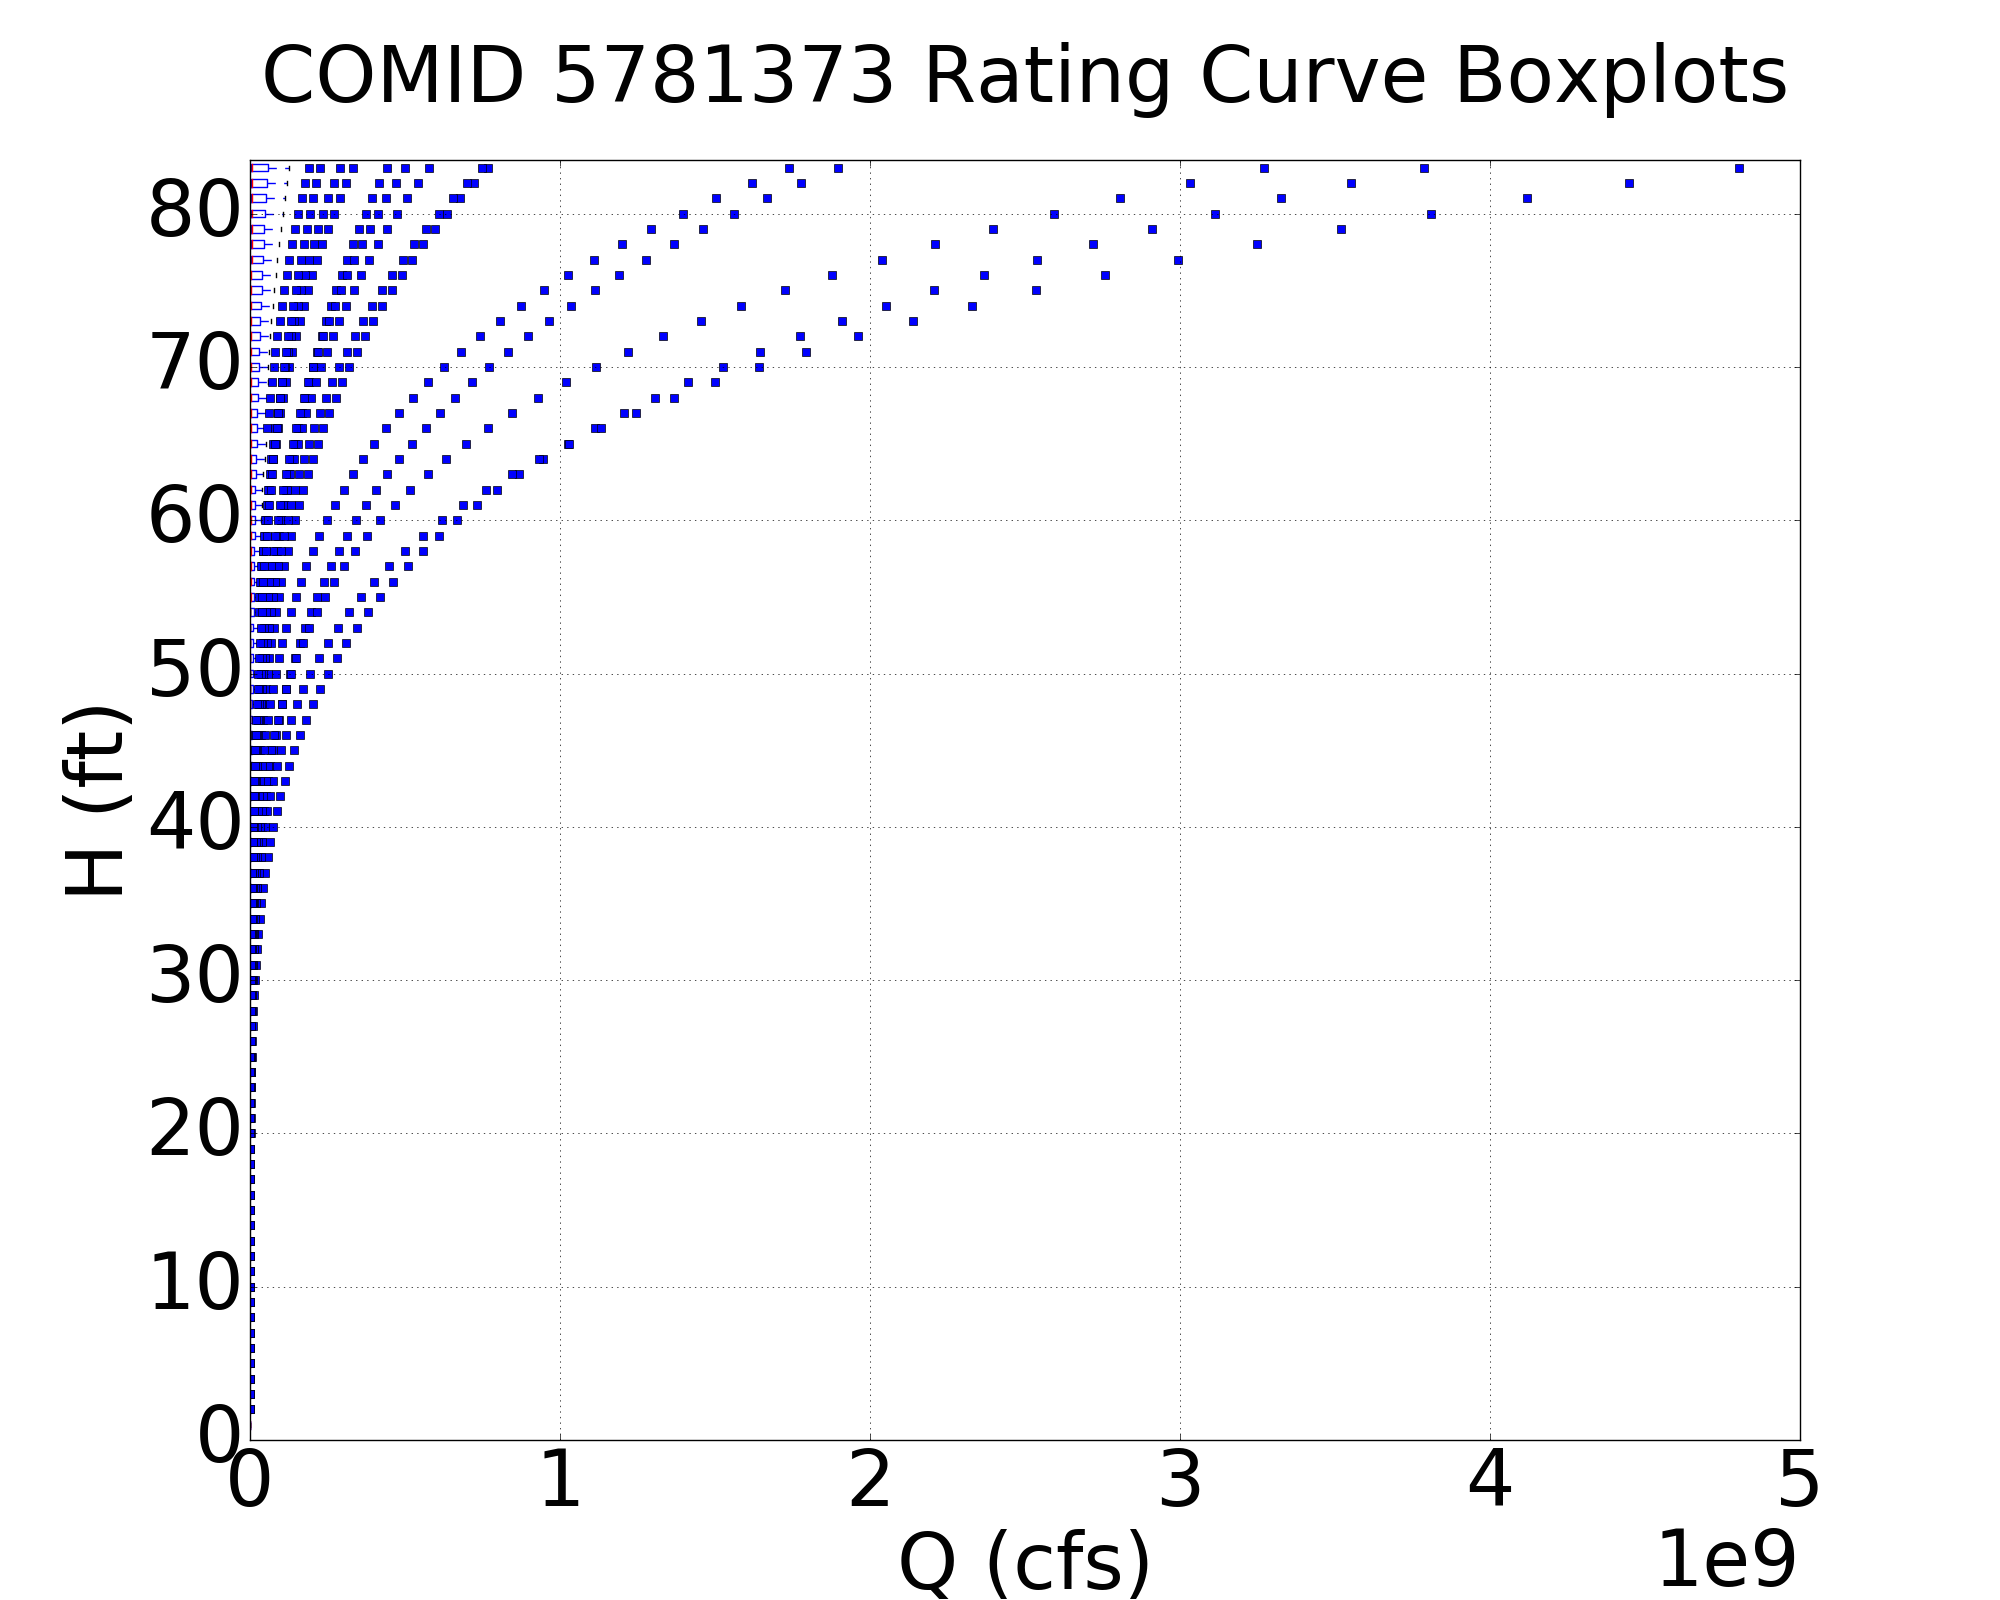
\includegraphics[keepaspectratio, width=\textwidth]{multi_boxplot_5781373.png}
  \caption{COMID 5781373 Boxplots}\label{fig:5781373_box}
\end{subfigure}
% \hspace*{\fill}
\begin{subfigure}{0.33\textwidth}
  \centering
  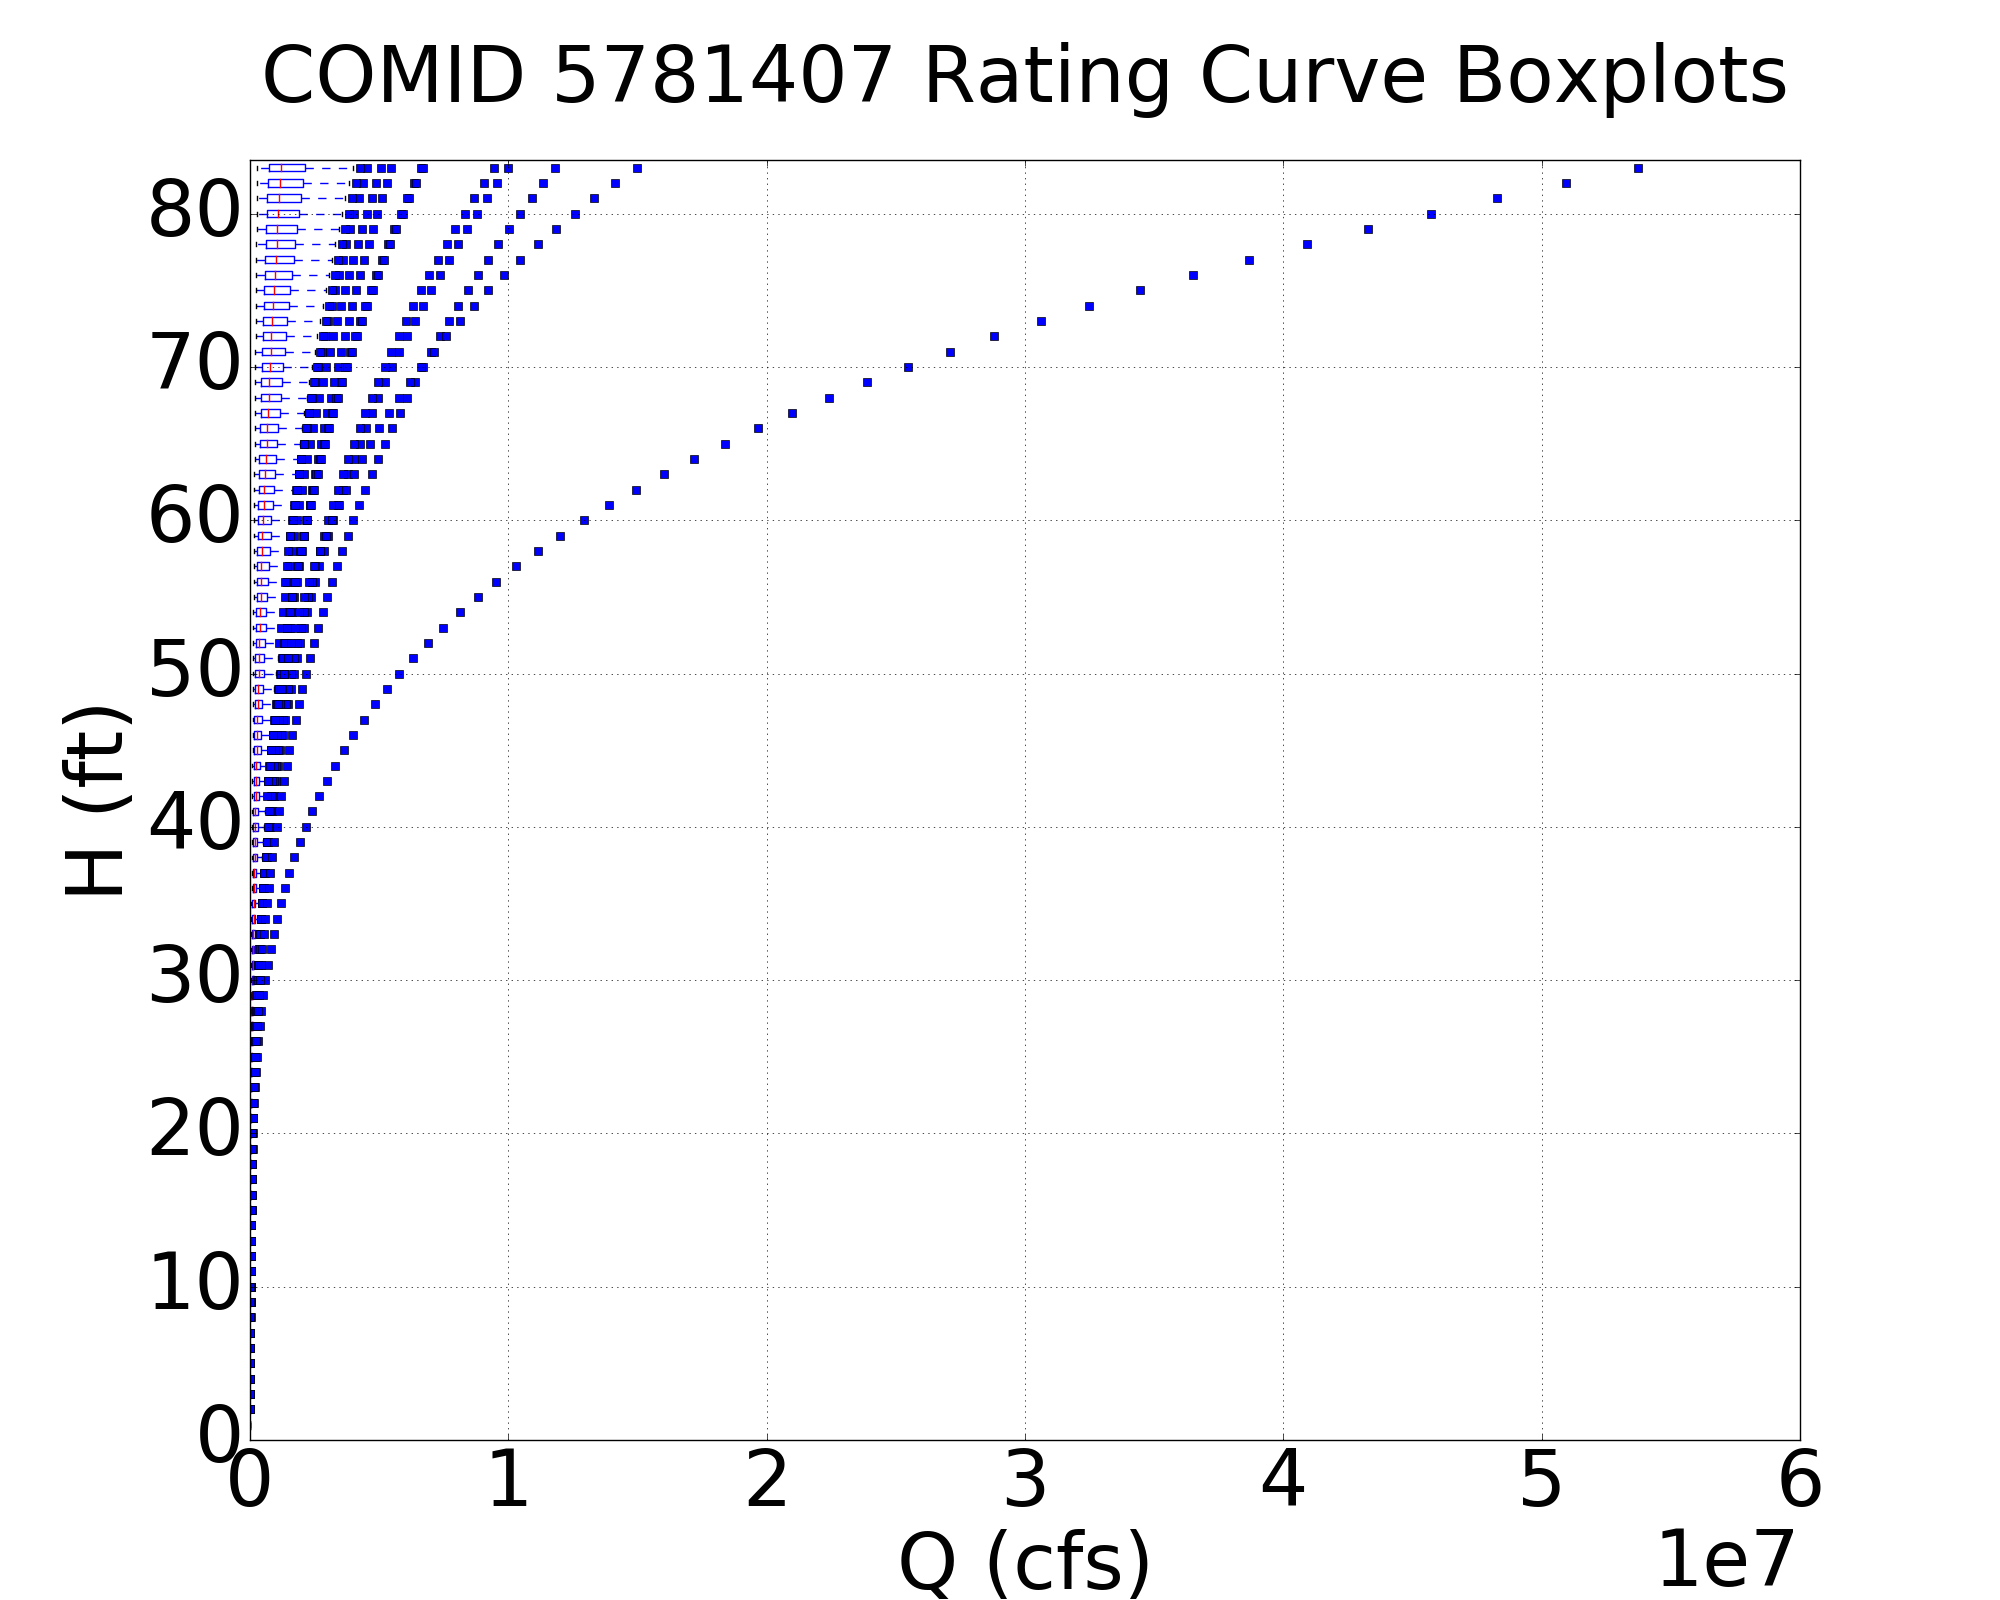
\includegraphics[keepaspectratio, width=\textwidth]{multi_boxplot_5781407.png}
  \caption{COMID 5781407 Boxplots}\label{fig:5781407_box}
\end{subfigure}
% \hspace*{\fill}
}
\caption{Boxplots showing the spread of discharge values in all HEC-RAS rating curves} \label{fig:hecrasboxplots}
\end{figure}

As is clearly shown in Figure \ref{fig:hecrasboxplots}, not only is there a large spread of data, but some COMIDs have incredibly large outliers. These outliers, which tend to appear more at higher stage heights, are likely related to the power-law regression used to fit the rating curves: as stage-height increases, discharge values of the power-law fit quickly trend towards infinity, thus producing some of the results seen in COMIDs 5781373 and 5781407.  

\subsection*{Rating Curves}

Rating curve results are shown below in Figure \ref{fig:ratingcurves} for the three COMIDs in question. Clearly the resistance functions don't exactly match a discharge-averaged rating curve, which makes perfect sense because they are roughness-averaged curves. Aside from that, it is unclear why the USGS and HEC-RAS curves seem to be in the lower ranges of the HEC-RAS curve spread. Rationally, this may mean that USGS gages are placed at wider cross-sections (where, generally, stage-height increases less as discharge increases). This may make sense from a field-installation and observation standpoint: data can be collected from much larger storms (ie. higher discharges) without the storm destroying the gage. Despite this seemingly rational explanation, there is no way of knowing whether this is true in practice or not (save viewing all of the USGS gages in the field). However, if this were known, there may be potential for generalizing the USGS rating curves for the reast of the nation, by taking into account where a USGS gage would be most likely placed and using the geometry of that particular cross-section as the USGS rating curve. This would not necessarily improve the accuracy of rating curves, but it would at least maintain consistency with the current USGS practices. 

\begin{figure}[h!]
\makebox[\linewidth][c]{
\begin{subfigure}{0.33\textwidth}
  \centering
  \includegraphics[keepaspectratio, width=\textwidth]{rc__comid_5781369_from_0_to_100.png}
  \caption{COMID 5781369 Curves}\label{fig:5781369_rc}
\end{subfigure}
% \hspace*{\fill}
\begin{subfigure}{0.33\textwidth}
  \centering
  \includegraphics[keepaspectratio, width=\textwidth]{rc__comid_5781373_from_0_to_100.png}
  \caption{COMID 5781373 Curves}\label{fig:5781373_rc}
\end{subfigure}
% \hspace*{\fill}
\begin{subfigure}{0.33\textwidth}
  \centering
  \includegraphics[keepaspectratio, width=\textwidth]{rc__comid_5781407_from_0_to_100.png}
  \caption{COMID 5781407 Curves}\label{fig:5781407_rc}
\end{subfigure}
% \hspace*{\fill}
}
\caption{Rating Curves from HAND, USGS, HEC-RAS, and the Resistance Function} \label{fig:ratingcurves}
\end{figure}

\subsection*{COMID 5781369 Rating Curve Sections, 5,000ft Lengths}

Below are some images of the rating curves for COMID 5781369 (Figure \ref{fig:5781369ratingcurves}) with the river channel split into 5,000ft lengths. The USGS, HAND, and Resistance Function curves shown are all at the entire stream-reach scale, whereas the HEC-RAS curves shown are only relevant to the scale in the image title (measured in percent-length, so 32 means 32\% along the stream length). These images have been created for all other stream reaches in the Onion Creek watershed containing both HEC-RAS cross-sections and USGS gage data, yet there were far too many images to efficiently and effectively display in this report. This particular COMID is one of the best performers of the group in terms of consistent profile-length HEC-RAS cross-sectional changes (meaning that the cross-sections seem to look similar in different sections of the stream reach). This ends up showing that the USGS rating curve matches up fairly nicely with the HEC-RAS cross-sections at that same location. Sadly, this is not the case for the other stream reaches analyzed; the majority of the other COMIDs experienced much more variability and no significant consistency amongst the data. Of note: the third segment of the reach cuts off at a profile percent-length of 96.64, and this is done because there were no further cross-sections along this stream reach.

\begin{figure}[h!]
\makebox[\linewidth][c]{
\begin{subfigure}{0.33\textwidth}
  \centering
  \includegraphics[keepaspectratio, width=\textwidth]{rc__comid_5781369_from_0_to_32.png}
  \caption{COMID 5781369, 0-32}\label{fig:5781369_rc}
\end{subfigure}
% \hspace*{\fill}
\begin{subfigure}{0.33\textwidth}
  \centering
  \includegraphics[keepaspectratio, width=\textwidth]{rc__comid_5781373_from_0_to_100.png}
  \caption{COMID 5781369, 32-64}\label{fig:5781373_rc}
\end{subfigure}
% \hspace*{\fill}
\begin{subfigure}{0.33\textwidth}
  \centering
  \includegraphics[keepaspectratio, width=\textwidth]{rc__comid_5781407_from_0_to_100.png}
  \caption{COMID 5781369, 64-97}\label{fig:5781407_rc}
\end{subfigure}
% \hspace*{\fill}
}
\caption{Boxplots showing the spread of discharge values in all HEC-RAS rating curves} \label{fig:5781369ratingcurves}
\end{figure}

\section*{Discussion}

The resistance function curves are not visibly relatable to the HAND and USGS curves. This is somewhat expected due to the two errors in these curves: USGS curves are highly localized and incredibly detailed for one particular cross-section of the stream reach, while HAND rating curves are generalized over the whole reach while assuming an approximate manning's roughness value of 0.05 (thus ignoring physical river characteristics entirely). 

Additionally, as shown by the scaling analysis, there are no clear and consistent trends with HEC-RAS cross-sections as associated with profile length. HEC-RAS cross-sections seem to change sporadically, and this high variability means that observing individual cross-sections is not a profitable pursuit. 

The HEC-RAS resistance function would likely be a more accurate representation of the stream reach as a whole than both the USGS and HAND methods, yet there is one considerable downfall to this methodology as well: despite the fact that these resistance functions take into account multiple cross-sections along each reach, the tremendously high cross-sectional variability makes it unlikely that even all the HEC-RAS cross-sections together could accurately represent the reach. Essentially this means that differentially-spaced cross-sections must be taken all along a reach (which is improbable and incredibly unlikely to ever occur), or a new way of generalizing stream characteristics at the reach scale --- without depending on cross-section data --- is necessary. 

\section*{Conclusions}

This comparrison has led to the conclusion that cross-sectional data, even in high density, is not particularly useful to collecting stream-reach-scale hydraulic properties. The new goal, then, is to generalize hydraulic properties accurately at the stream-reach-scale, which is also the intent behind the HAND methodology. As such, this report confirms the validity of the HAND rating curve approach for hydraulic property generalizations, ultimately enabling accurate flood extent predictions for all CONUS stream reaches. 

\printbibliography

\end{document}